\chapter{Approach}

\section{Introduction}
This chapter presents the approach adopted in this dissertation for lyric reconstruction from bag-of-words style constraints. The proposed method is inspired by LyCon, but extends this general idea through a prompt-based framework that combines lexical cues, song metadata, and affective information derived from valence and arousal. Rather than treating lyric generation as an unconstrained text generation task, the approach represents each song through a structured set of features that can be used to guide the language model towards outputs that better reflect the source song.

The chapter explains how songs are selected and represented, how lexical vocabularies are extracted from the reference lyrics, how emotional information is incorporated through mood representations, and how different prompt designs are used to impose varying levels of control over the generated lyrics. It also outlines the evaluation strategy used to assess the resulting outputs. Together, these components form the methodological basis for the experimental study presented in the next chapter.

\section{Overview of the Proposed Approach}

The proposed approach is organised as a prompt-based lyric reconstruction pipeline. Rather than generating lyrics from unconstrained instructions, each song is first transformed into a structured representation that captures information about its identity, affective characteristics, and lexical content. This representation is then used to construct prompts that guide the language model towards outputs that more closely reflect the source song.

At a high level, the process begins with song selection from the Music4All dataset, followed by the preparation of the relevant metadata and reference lyrics. The lyrics are then processed to extract vocabulary cues that act as bag-of-words style constraints, while valence and arousal values are used to derive a compact mood representation. These lexical and affective features are combined with song metadata to form prompt inputs, from which multiple prompt variants are constructed. Each prompt variant represents a different level or style of control, allowing the dissertation to compare how structure, lexical guidance, and frequency information affect lyric reconstruction.

Once the prompts are constructed, the selected language model generates a reconstructed lyric for each song. The outputs are then evaluated against the reference lyrics using a set of structural, lexical, diversity, and semantic similarity measures.

\begin{figure}[H]
    \centering
    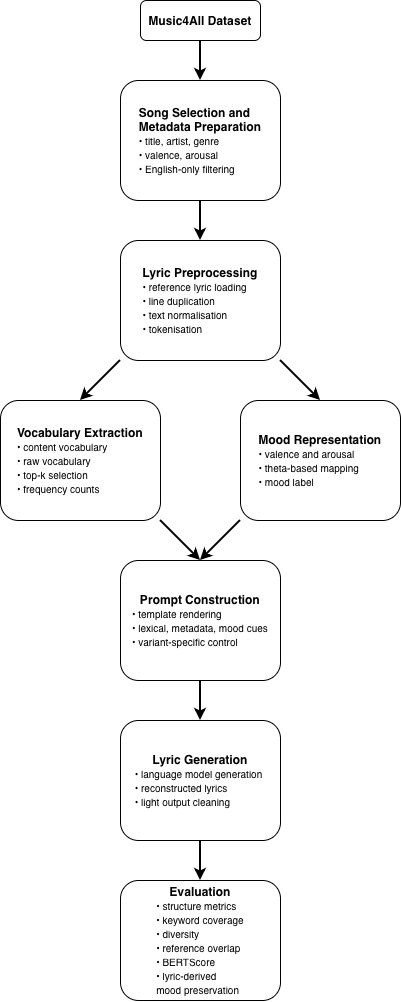
\includegraphics[width=0.60\textwidth]{figures/approach-pipeline.png}
    \caption{Overview of the proposed lyric reconstruction pipeline.}
    \label{fig:approach_pipeline}
\end{figure}


Figure~\ref{fig:approach_pipeline} summarises the overall pipeline used in this dissertation. The following sections describe each stage of the approach in more detail.

\section{Dataset Selection and Song Representation}

This dissertation uses the Music4All dataset as the basis for the lyric reconstruction task. Although the project is inspired by LyCon, the experiments are not conducted directly on LyCon's released reconstructed lyrics. An initial attempt was made to consider LyCon's published outputs as the basis for evaluation. However, the released material does not provide a sufficiently controlled setting for systematic comparison against original reference lyrics across multiple prompt conditions. In practice, this makes it difficult to construct a consistent reconstruction benchmark in which generated outputs can be evaluated against paired ground-truth lyrics under a shared experimental design.

For this reason, Music4All was selected as the primary dataset for the study. Music4All provides both lyric files and song-level metadata, making it possible to build a reproducible lyric reconstruction pipeline with explicit reference texts for evaluation. This is particularly important in the present dissertation, where the objective is not only to produce reconstructed lyrics, but also to compare different prompt-control strategies against the original lyrics in a consistent and measurable way.

From the available metadata, the approach uses the song title, artist name, genre-related information, and affective features derived from valence and arousal. In the Music4All dataset, arousal is approximated using the available energy measure, allowing the dataset to be aligned with the valence-arousal framing used by LyCon. In addition, the reference lyrics are used as the source from which lexical constraints are derived. This allows the reconstruction task to be framed as generation from an informative but incomplete representation of the original song, rather than direct reproduction of the full lyrics. Music4All is therefore well suited to the construction of a LyCon-inspired baseline condition, while also supporting the broader comparative experiments introduced in later chapters.

To ensure consistency across the dataset, only songs with the required metadata and available lyric content are retained. The dataset is also restricted to English-language songs so that lexical extraction and evaluation can be applied more reliably within a single language setting. Songs with missing titles, artists, genre information, valence, arousal, or usable lyric data are excluded from the final sample. In addition, the sampling procedure is controlled through a fixed random seed so that the same song set can be reused across experimental conditions.

Each retained song is therefore represented as a structured input instance consisting of its metadata, affective attributes, and lyric-derived vocabulary cues. This representation forms the basis for prompt construction in the later stages of the pipeline. By transforming each song into a controlled set of lexical and contextual signals, the approach enables a systematic comparison of different prompt strategies for lyric reconstruction.

\section{Preprocessing and Vocabulary Extraction}

The preprocessing stage converts the reference lyrics of each selected song into a controlled lexical representation that can be used for prompting. This step is central to the dissertation, since the reconstruction task is framed not as generation from the full original lyrics, but as generation from a reduced bag-of-words style representation derived from them. The objective of preprocessing is therefore to transform the raw lyric text into a consistent and informative set of lexical cues while preserving the distinctions required for the later experimental conditions.

For each selected song, the corresponding lyric file is first loaded and normalised into a consistent text format. As lyrics often contain repeated choruses, hooks, and refrains, the preprocessing pipeline applies line deduplication before vocabulary extraction. This means that repeated lines are only counted once when constructing the lexical representation. The purpose of this step is to reduce the influence of repeated lyrical structure on the vocabulary signal, ensuring that highly repeated sections do not dominate the lexical cues simply because they occur multiple times in the original song.

The normalised lyric text is then tokenised into lowercase alphabetic word tokens, providing a simple and consistent lexical representation across songs. At this stage, the pipeline produces two different token representations from the same lyric source. The first is a raw token stream, which retains a broad surface-level representation of the lyrics. The second is a content-based token stream, which applies stopword removal and a minimum token length threshold in order to retain more semantically informative words. In the implementation used in this dissertation, content vocabulary extraction removes common function words and filters tokens shorter than three characters, while raw vocabulary extraction retains these more literal surface-level elements. These two token streams form the basis for the later comparison between raw and content vocabulary prompting.

After tokenisation, frequency counts are computed over the extracted tokens in order to identify the most salient lexical items in each song. From these frequency counts, top-k vocabulary lists are produced, where \(k\) is configurable depending on the experimental condition. This makes it possible to compare smaller and larger lexical budgets, such as top-20, top-50, and top-100 vocabularies. In addition to plain vocabulary lists, the pipeline also stores frequency-annotated vocabulary strings in the form \texttt{word:count}. This allows later prompt variants to make use not only of lexical presence, but also of approximate lexical importance.

The output of this stage is therefore a structured lexical representation for each song, including both raw and content-based vocabulary forms, as well as their associated frequency information. Songs for which usable lyrics or derived vocabulary representations cannot be obtained are excluded from the final dataset. These extracted lexical cues form the core bag-of-words style constraints used for prompt construction throughout the remainder of the lyric reconstruction pipeline.

\section{Content Vocabulary and Raw Vocabulary Representations}

A central design choice in this dissertation is the use of two different lexical representations derived from the same reference lyrics: content vocabulary and raw vocabulary. Although both are extracted from the original song text, they reflect different assumptions about what kind of lexical information is most useful for lyric reconstruction. Because the two representations are generated from the same lyric source, the comparison between them is controlled at the level of the underlying song text, with the primary difference lying in how the lexical signal is filtered and represented. This distinction allows the dissertation to examine whether reconstruction benefits more from a semantically focused representation or from a broader surface-level representation of the source lyrics.

The content vocabulary representation is intended to capture the more informative lexical core of a song. By removing common function words and filtering out very short tokens, this representation emphasises words that are more likely to contribute to theme, imagery, and lyrical content. In the implementation used here, content vocabulary extraction applies a lyric-aware stopword list and a minimum token length threshold of three characters. This reduces the influence of highly frequent but less informative words, producing a more selective bag-of-words signal. Such a representation is particularly suitable for prompt conditions that aim to preserve semantic direction while leaving the language model some flexibility in phrasing and structure.

By contrast, the raw vocabulary representation retains a wider range of lexical material from the original lyrics. This includes function words, short tokens, and other surface-level elements that are excluded from the content-based representation. As a result, the raw vocabulary may preserve aspects of the original lexical texture more directly, potentially encouraging outputs that more closely resemble the wording of the reference song. However, this broader representation may also introduce noise, as highly frequent but low-information words can dominate the lexical signal and reduce its semantic selectivity.

Table~\ref{tab:raw_content_vocab_example} illustrates the difference between the two representations using one song from the experimental sample.

\begin{table}[ht]
\centering
\caption{Example comparison of raw and content vocabulary representations for Stevie Wonder's ``Do I Do''.}
\label{tab:raw_content_vocab_example}
\begin{tabular}{p{0.28\textwidth} p{0.62\textwidth}}
\hline
Representation & Top vocabulary terms \\
\hline
Raw vocabulary & do, i, you, love, your, my, the, to, when, for \\
Content vocabulary & love, when, what, blow, some, girl, kisses, all, chocolate, been \\
\hline
\end{tabular}
\end{table}

The example shows how the raw representation preserves more surface-level lyric material, while the content representation suppresses frequent low-information terms and foregrounds words that are more useful as semantic constraints.

Both vocabulary forms are represented not only as plain word lists but also as frequency-ranked lexical cues. This means that the distinction between raw and content vocabulary can influence both the set of words presented to the language model and the relative prominence assigned to those words in frequency-aware prompt variants. In practical terms, the selected vocabulary strategy determines the lexical fields used for prompt construction, making the representation choice a direct component of the reconstruction process rather than a purely descriptive preprocessing decision.

The comparison between content vocabulary and raw vocabulary is therefore methodologically important. It allows the dissertation to test whether lyric reconstruction is better supported by a cleaner and more semantically focused lexical representation, or by a more literal representation that more closely reflects the surface form of the original lyrics. This distinction also provides a principled basis for one of the core experimental comparisons in the study. More broadly, it helps clarify how the type of lexical constraint influences the balance between fluency, thematic consistency, and reconstruction fidelity in prompt-based lyric generation.

\section{Mood Representation from Valence and Arousal}

In addition to lexical constraints, the proposed approach incorporates affective information into the lyric reconstruction process. This is motivated by the LyCon framework, which uses valence and arousal as part of its representation of lyrical emotion. Valence broadly describes the positivity or negativity of a song, while arousal describes its level of energy or activation. Together, these dimensions provide a compact way to represent the emotional character of a song and to condition the generated lyrics accordingly.

The Music4All dataset provides valence values together with an energy feature obtained from Spotify metadata. In this dissertation, the energy feature is treated as a proxy for arousal, allowing the dataset to be aligned with the valence-arousal representation used in LyCon-inspired lyric reconstruction. Where necessary, values on a unit scale are centred so that the affective space can be interpreted around a neutral origin. Each song is therefore represented as a point in a two-dimensional valence-arousal space.

To convert this continuous affective representation into a promptable form, the approach computes the angular position of each song in the valence-arousal plane. This follows the same general principle as LyCon, where the emotional position of a song is represented by its direction in the valence-arousal space. The angle is calculated using the two-argument arctangent function:

\[
\theta = \operatorname{atan2}(a, v)
\]

where \(v\) represents the centred valence value and \(a\) represents the centred arousal value. Following the LyCon-style use of the valence-arousal plane, the resulting angle \(\theta\) is mapped into one of 12 mood sectors, producing a discrete mood label such as \textit{happy}, \textit{excited}, \textit{calm}, or \textit{sad}. Figure~\ref{fig:mood_sector_mapping} illustrates this mood-sector mapping.

\begin{figure}[H]
\centering
\resizebox{0.84\textwidth}{!}{%
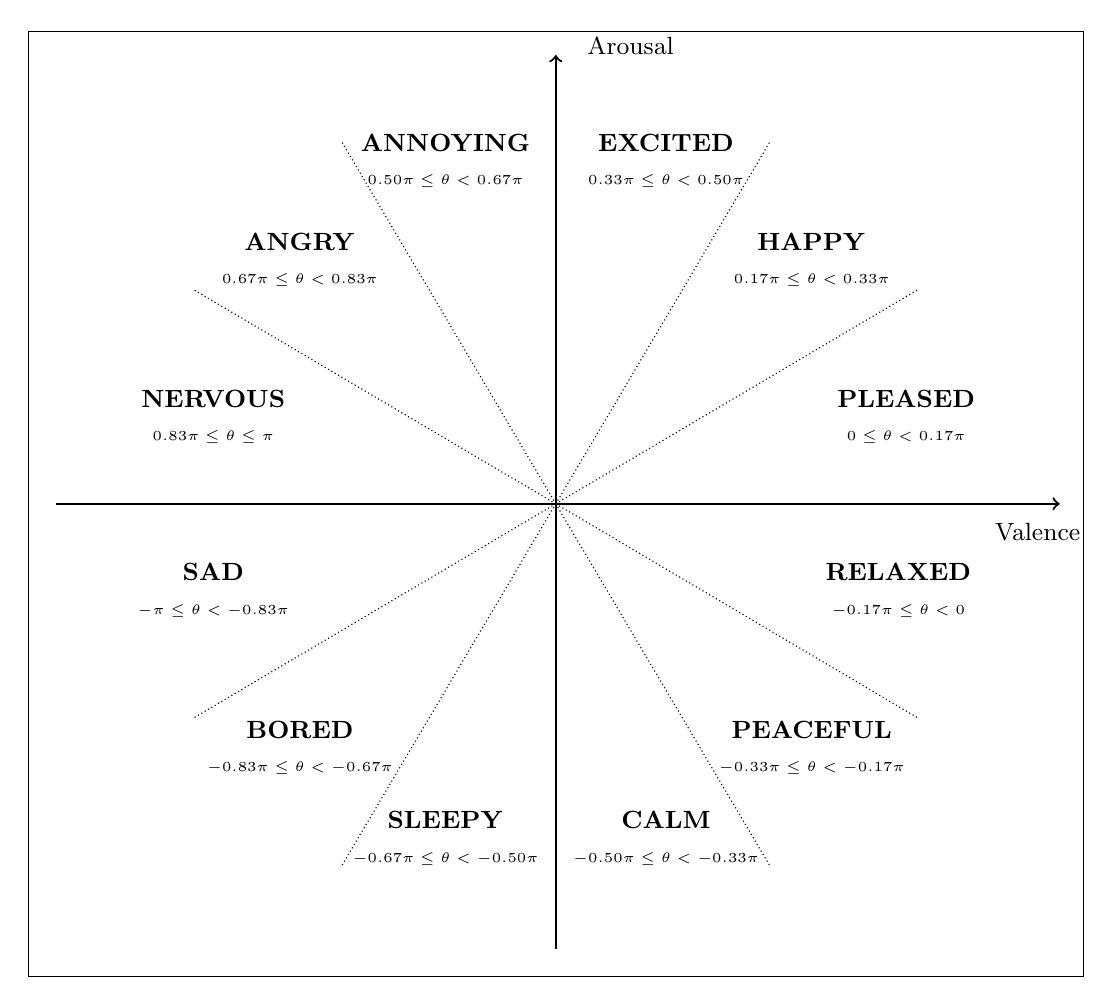
\begin{tikzpicture}

\draw[black] (-6.70,-6.00) rectangle (6.70,6.00);

\draw[->, thick] (-6.35,0) -- (6.40,0);
\draw[->, thick] (0,-5.65) -- (0,5.70);

\node[font=\small] at (0.95,5.82) {Arousal};
\node[font=\small] at (6.12,-0.35) {Valence};

\foreach \a in {-180,-149.4,-120.6,-90,-59.4,-30.6,0,30.6,59.4,90,120.6,149.4,180} {
    \draw[densely dotted] (0,0) -- (\a:5.35);
}

\node[align=center] at (4.45,1.1) {{\small \textbf{PLEASED}}\\{\tiny \(0 \leq \theta < 0.17\pi\)}};
\node[align=center] at (3.25,3.10) {{\small \textbf{HAPPY}}\\{\tiny \(0.17\pi \leq \theta < 0.33\pi\)}};
\node[align=center] at (1.4,4.35) {{\small \textbf{EXCITED}}\\{\tiny \(0.33\pi \leq \theta < 0.50\pi\)}};
\node[align=center] at (-1.4,4.35) {{\small \textbf{ANNOYING}}\\{\tiny \(0.50\pi \leq \theta < 0.67\pi\)}};
\node[align=center] at (-3.25,3.10) {{\small \textbf{ANGRY}}\\{\tiny \(0.67\pi \leq \theta < 0.83\pi\)}};
\node[align=center] at (-4.35,1.1) {{\small \textbf{NERVOUS}}\\{\tiny \(0.83\pi \leq \theta \leq \pi\)}};

\node[align=center] at (-4.35,-1.1) {{\small \textbf{SAD}}\\{\tiny \(-\pi \leq \theta < -0.83\pi\)}};
\node[align=center] at (-3.25,-3.10) {{\small \textbf{BORED}}\\{\tiny \(-0.83\pi \leq \theta < -0.67\pi\)}};
\node[align=center] at (-1.4,-4.25) {{\small \textbf{SLEEPY}}\\{\tiny \(-0.67\pi \leq \theta < -0.50\pi\)}};
\node[align=center] at (1.4,-4.25) {{\small \textbf{CALM}}\\{\tiny \(-0.50\pi \leq \theta < -0.33\pi\)}};
\node[align=center] at (3.25,-3.10) {{\small \textbf{PEACEFUL}}\\{\tiny \(-0.33\pi \leq \theta < -0.17\pi\)}};
\node[align=center] at (4.35,-1.1) {{\small \textbf{RELAXED}}\\{\tiny \(-0.17\pi \leq \theta < 0\)}};

\end{tikzpicture}%
}
\caption{Valence-arousal mood sector mapping adapted from LyCon.}
\label{fig:mood_sector_mapping}
\end{figure}

The resulting mood label is inserted into the prompt templates as an affective cue, allowing the language model to receive not only lexical and metadata information, but also a compact description of the intended emotional tone. This mood representation is not intended to provide a complete model of lyrical emotion. Instead, it serves as a lightweight conditioning signal that allows the generated lyrics to be guided by the affective metadata available for each song. Combined with the vocabulary cues described in the previous sections, the mood label helps define the target song representation used throughout the prompt-based reconstruction pipeline.

\section{Prompt Design Strategy}

Prompt design is the central mechanism through which the reconstruction task is controlled in this dissertation. Once each song has been represented through its metadata, lyric-derived vocabulary, and affective mood label, these components are inserted into prompt templates that instruct the language model to generate a reconstructed lyric. The prompts therefore act as the interface between the reduced song representation and the generative model. Rather than asking the model to generate lyrics freely, the prompt provides a constrained description of the source song and specifies how strongly the model should use the available cues.

The prompt design strategy is experimental in nature. Different prompt templates are used to impose different levels and types of control over the generation process. This makes it possible to investigate how reconstruction quality changes when the model is given more explicit structural guidance, stronger lexical requirements, frequency information, or a larger vocabulary budget. In this way, prompt design is not treated simply as an implementation detail, but as the main variable through which the dissertation studies lyric reconstruction from bag-of-words style inputs.

Several dimensions of control are considered. The first is lexical control, which concerns the extent to which the model is instructed to use the vocabulary extracted from the reference lyrics. In some variants, the vocabulary is presented as a central requirement, while in others it is framed more loosely as inspiration. The second is structural control, where the prompt may require the generated lyric to follow a specific organisation such as Verse 1, Chorus, Verse 2, and Chorus. This allows the experiments to examine whether explicit structural instructions improve the formal organisation of the generated lyrics.

A third dimension is frequency-aware control. Since the preprocessing stage stores not only vocabulary lists but also frequency counts, some prompt variants provide the model with information about which words were more prominent in the reference lyrics. The purpose of this is to test whether approximate frequency information helps the model preserve more important lexical cues rather than treating all supplied words equally. A fourth dimension is vocabulary representation, which distinguishes between content vocabulary and raw vocabulary. This comparison tests whether a cleaner semantic vocabulary or a broader surface-level vocabulary provides a better reconstruction signal.

The prompt design also varies the size of the vocabulary supplied to the model. By comparing top-20, top-50, and top-100 vocabulary settings, the experiments examine whether a smaller lexical budget produces more focused outputs, or whether a larger vocabulary helps the model remain closer to the reference lyric. Finally, the prompts vary in overall strictness. Minimal-control prompting gives the model more freedom, while strong-control prompting explicitly requires prominent vocabulary use, structural compliance, and coherent emotional expression.

This design allows the dissertation to compare prompt strategies under a controlled experimental setting. Since the same song sample is used across the final runs, differences in the generated outputs can be interpreted in relation to the prompt conditions rather than changes in the underlying dataset. The following section describes the specific prompt variants and control levels used in the experiments.

\section{Prompt Variants and Control Levels}

The experimental design includes a set of prompt variants that differ in the type and strength of control imposed on the language model. Each variant uses the same general song representation, but changes how the available information is presented to the model. This makes it possible to compare reconstruction behaviour across different prompt-control settings while keeping the underlying song sample consistent.

Table~\ref{tab:prompt_variants} summarises the main prompt variants used in the final experiments.

\begin{table}[ht]
\centering
\renewcommand{\arraystretch}{1.45}
\caption{Summary of prompt variants used in the lyric reconstruction experiments.}
\label{tab:prompt_variants}
\begin{tabular}{
p{0.05\textwidth}
>{\raggedright\arraybackslash}p{0.20\textwidth}
>{\raggedright\arraybackslash}p{0.24\textwidth}
>{\raggedright\arraybackslash}p{0.41\textwidth}
}
\hline
No. & Prompt variant & Main control type & Purpose \\
\hline
1 & Baseline LyCon-style & Metadata, mood, content vocabulary & Provides a baseline reconstruction condition inspired by LyCon-style prompting. \\
2 & Structured & Explicit lyric structure & Tests whether verse and chorus instructions improve formal organisation. \\
3 & Frequency-aware & Structure and word frequency cues & Tests whether frequency information helps prioritise important vocabulary. \\
4 & Raw vocabulary & Surface-level vocabulary & Tests whether retaining function words and short tokens improves reconstruction. \\
5 & Top-20 vocabulary & Reduced lexical budget & Tests whether a compact vocabulary signal produces more focused outputs. \\
6 & Top-100 vocabulary & Expanded lexical budget & Tests whether a larger vocabulary signal improves reference similarity. \\
7 & Minimal control & Loose vocabulary guidance & Tests the effect of giving the model greater freedom. \\
8 & Strong control & Structure, vocabulary, and frequency constraints & Tests the most constrained reconstruction setting. \\
\hline
\end{tabular}
\renewcommand{\arraystretch}{1.0}
\end{table}




\subsection{Baseline LyCon-Style Prompting}

The baseline prompt is designed to provide a LyCon-inspired reconstruction condition. It uses the song title, artist name, genre, mood label, and lyric-derived content vocabulary as the main input cues. The prompt asks the model to compose lyrics in a style reminiscent of the given artist, representing the derived mood label, and using the supplied vocabulary. This establishes a simple reconstruction setting in which the model receives both contextual and lexical information, but is not given explicit structural requirements.

This baseline is important because it provides a reference point for evaluating the later prompt variants. Since it includes the main song-level cues used throughout the dissertation, it represents the minimum controlled reconstruction condition against which additional forms of prompt control can be compared. However, because it does not enforce verse or chorus organisation, the generated structure is left largely to the language model.

\subsection{Structured Prompting}

The structured prompt extends the baseline by adding explicit instructions about lyric organisation. In addition to genre, artist, mood label, title, and vocabulary, the model is instructed to structure the output into Verse 1, Chorus, Verse 2, and Chorus. The purpose of this variant is to test whether a clear structural template improves the formal organisation of the generated lyrics.

This condition is motivated by the observation that lyric reconstruction involves not only recovering relevant words, but also arranging them into a recognisable lyrical form. A generated output may contain appropriate vocabulary but still be weak as a lyric if it lacks coherent sections or repeated chorus-like material. Structured prompting therefore tests whether formal constraints help the model produce outputs that better resemble conventional song lyrics.

\subsection{Frequency-Aware Prompting}

The frequency-aware prompt builds on the structured condition by adding frequency information for the supplied vocabulary. Instead of presenting only a list of words, this variant also provides approximate word counts in the form \texttt{word:count}. These counts are derived from the reference lyrics during preprocessing and are intended to indicate which lexical items were more prominent in the source song.

The purpose of frequency-aware prompting is to test whether the model can make more effective use of the vocabulary when given information about relative lexical importance. In a plain vocabulary list, all words are presented with equal weight, even though some may be central to the original lyric while others appear only once. By providing frequency cues, the prompt encourages the model to reuse more important words more prominently while still maintaining fluency and coherence.

\subsection{Raw Vocabulary Prompting}

The raw vocabulary prompt uses the same general baseline style but changes the vocabulary representation. Instead of using content vocabulary, it uses raw vocabulary extracted from the reference lyrics. This means that the supplied vocabulary may include function words, short tokens, and other surface-level lexical material that would normally be removed in the content vocabulary condition.

This variant tests whether a broader and more literal vocabulary representation provides a better reconstruction signal. Raw vocabulary may help preserve aspects of the original lyric's surface form because it contains common words and phrasing elements that are filtered out of the content-based representation. However, it may also introduce noise by giving the model less semantically selective lexical cues. The raw vocabulary condition is therefore used to examine the tradeoff between surface-level fidelity and lexical informativeness.

\subsection{Vocabulary Size Variants}

Two additional baseline-style variants are used to examine the effect of vocabulary size. The top-20 condition provides only the twenty most frequent content vocabulary terms from each reference lyric, while the top-100 condition provides a much larger set of lexical cues. These variants allow the dissertation to examine how the size of the bag-of-words representation affects reconstruction behaviour.

The top-20 condition represents a compact lexical budget. It gives the model only the most prominent words and therefore tests whether a smaller set of high-salience cues is sufficient to guide reconstruction. This may encourage more focused outputs, but it may also omit important secondary details from the original lyric. By contrast, the top-100 condition provides a broader lexical representation. This may help the generated output remain closer to the reference lyric, but it may also make the prompt less focused or harder for the model to satisfy fully.

Together, these conditions allow the dissertation to investigate whether lyric reconstruction benefits more from concise lexical guidance or from a larger vocabulary signal.

\subsection{Minimal Control Prompting}

The minimal-control prompt is designed to reduce the strength of the lexical constraint. In this condition, the vocabulary is presented only as optional inspiration rather than as a required set of words to use. The model is still given metadata and mood information, but it is allowed more freedom in deciding whether and how to incorporate the supplied vocabulary.

This variant provides a useful contrast to the more controlled prompt conditions. If the model performs well under minimal control, this would suggest that detailed lexical constraints may not be necessary for generating plausible lyrics. If performance decreases, this would suggest that stronger prompt control may be important for reconstructing lyrics from reduced song representations. The minimal-control condition therefore helps clarify the role of explicit lexical guidance in the reconstruction process.

\subsection{Strong Control Prompting}

The strong-control prompt represents the most constrained condition in the experimental design. It combines explicit structural requirements, prominent vocabulary use, and frequency-aware lexical guidance. The model is instructed to structure the output into Verse 1, Chorus, Verse 2, and Chorus, to use many of the supplied vocabulary words explicitly, and to reuse important words where natural.

This condition is designed to test whether combining multiple forms of control leads to stronger reconstruction behaviour. Unlike the minimal-control condition, which gives the model substantial freedom, the strong-control prompt makes the reconstruction objective more explicit. It therefore represents the strongest attempt in the dissertation to guide the language model using the reduced song representation. Comparing this variant with the baseline, structured, and frequency-aware conditions allows the experiments to examine whether stronger control improves reconstruction, or whether excessive constraint introduces tradeoffs such as repetition or reduced naturalness.

\section{Lyric Generation Procedure}

After the prompt variants are constructed, they are used to generate reconstructed lyrics for each song in the experimental sample. Each final prompt condition is applied to the same set of 50 songs, ensuring that the outputs from different runs can be compared under a consistent dataset. For each song and prompt variant, the language model generates one reconstructed lyric using the corresponding prompt template and song representation.

The generation stage uses GPT-4o mini as the language model. This model is treated as a fixed generation component across the experiments, while the prompt design is varied between conditions. Keeping the model constant is important because it allows differences in the generated outputs to be interpreted primarily in relation to the prompt strategy rather than changes in model architecture or model capability.

For each run, the generated output is saved together with the song metadata, prompt input, prompt version, model name, and timestamp. The pipeline also stores a snapshot of the configuration used for the run, allowing the experimental conditions to be traced and reproduced. This includes information such as the vocabulary strategy, vocabulary size, prompt template, and whether structural constraints or frequency cues are used. By storing these files separately for each run, the pipeline maintains a clear record of how each output was produced.

A light output-cleaning step is applied after generation. This step removes obvious wrapper text such as introductory phrases, explanations, or closing remarks if they are produced by the language model. However, the generated lyric itself is not rewritten or manually corrected. This is important because the evaluation should reflect the model output produced under each prompt condition rather than a human-edited version of the text.

The same generation procedure is used across all final prompt variants. As a result, the main experimental difference between runs lies in the information and constraints provided through the prompt. This supports a controlled comparison of how lexical guidance, structural requirements, frequency information, vocabulary size, and prompt strictness influence lyric reconstruction.

\begin{table}[H]
\centering
\caption{Summary of the lyric generation setup.}
\label{tab:generation_setup}
\begin{tabular}{p{0.35\textwidth} p{0.50\textwidth}}
\hline
Component & Setting \\
\hline
Language model & GPT-4o mini \\
Songs per run & 50 \\
Outputs per song & One reconstructed lyric per prompt variant \\
Controlled variable & Prompt design \\
Stored run files & Prompt dataset, generated outputs, configuration snapshot, evaluation files \\
\hline
\end{tabular}
\end{table}


\section{Evaluation Strategy}

The generated lyrics are evaluated using a set of automatic metrics designed to capture different aspects of lyric reconstruction quality. Since lyric reconstruction cannot be assessed using a single measure, the evaluation strategy considers structural form, lexical adherence, similarity to the reference lyrics, diversity, repetition, and auxiliary mood preservation. These metrics are used together to provide a broader picture of how different prompt-control strategies affect the generated outputs.

The evaluation is performed against the reference lyrics from the Music4All dataset. However, the aim is not to reward exact copying of the original lyrics. Instead, the metrics are used to examine whether the generated lyrics preserve important characteristics of the source song representation, such as its vocabulary, structure, and affective cues, while still producing coherent lyric text.

\begin{table}[H]
\centering
\renewcommand{\arraystretch}{1.25}
\caption{Summary of evaluation dimensions used in the dissertation.}
\label{tab:evaluation_dimensions}
\begin{tabular}{
>{\raggedright\arraybackslash}p{0.26\textwidth}
>{\raggedright\arraybackslash}p{0.32\textwidth}
>{\raggedright\arraybackslash}p{0.32\textwidth}
}
\hline
Evaluation dimension & Example metrics & Purpose \\
\hline
Structural form & Section count, structure score, order match & Measures whether outputs follow song-like organisation. \\
Lexical adherence & Keyword coverage, weighted coverage, keyword density & Measures use of supplied vocabulary cues. \\
Reference similarity & Jaccard, unigram overlap, bigram overlap, BERTScore & Measures similarity to the reference lyrics. \\
Diversity and repetition & Distinct n-grams, type-token ratio, repeated line ratio & Measures variety and excessive repetition. \\
Mood preservation & Classifier-based mood prediction, Warriner VA distance & Provides auxiliary affective comparison. \\
\hline
\end{tabular}
\renewcommand{\arraystretch}{1.0}
\end{table}

\subsection{Structural Evaluation}

Structural evaluation measures whether the generated lyrics resemble a recognisable song-like form. This is particularly important for prompt variants that explicitly request sections such as Verse 1, Chorus, Verse 2, and Chorus. The evaluation therefore includes measures such as line count, section count, structure score, and section order match.

The section-based metrics are used to assess whether generated outputs contain the expected lyrical divisions and whether these divisions appear in the intended order. This allows the structured and strong-control prompt variants to be compared against less constrained variants. A generated lyric may contain relevant vocabulary but still be structurally weak if it lacks clear sections or does not follow the requested verse-chorus organisation. Structural evaluation therefore captures an aspect of reconstruction quality that is not measured by lexical overlap alone.

The evaluation also records the length ratio between the generated lyric and the reference lyric. This provides a basic indication of whether generated outputs are substantially shorter or longer than the original lyric text.

\subsection{Lexical Adherence Evaluation}

Lexical adherence evaluation measures how effectively the generated lyrics use the vocabulary supplied in the prompt. Since the reconstruction task is based on bag-of-words style constraints, this is one of the central evaluation dimensions in the dissertation. The main lexical metrics include keyword coverage, top keyword coverage, weighted keyword coverage, and keyword density.

Keyword coverage measures the proportion of supplied vocabulary words that appear in the generated lyric. Top keyword coverage focuses on the highest-ranked vocabulary terms, while weighted keyword coverage takes frequency information into account when available. This allows the evaluation to distinguish between outputs that use only minor vocabulary terms and outputs that preserve more prominent words from the reference lyric. Keyword density is used to examine how much of the generated text consists of supplied vocabulary words. Title token coverage is also recorded to indicate whether important words from the song title are reflected in the generated output.

Together, these metrics help assess whether the language model follows the lexical constraints provided by each prompt variant. They are especially useful for comparing minimal-control, baseline, frequency-aware, and strong-control prompts.

\subsection{Reference Similarity Evaluation}

Reference similarity evaluation measures the degree of overlap between the generated lyric and the original reference lyric. This includes lexical overlap metrics such as reference Jaccard similarity, unigram precision, unigram recall, and bigram overlap. These measures provide an indication of how closely the generated output resembles the reference lyric at the word and phrase level.

In addition to surface-level overlap, BERTScore is used as a semantic similarity measure. BERTScore compares generated and reference lyrics using contextual language representations, allowing the evaluation to capture forms of similarity that may not rely on exact word matching. This is useful because a generated lyric may express related themes or emotional content while using different wording from the original lyric.

These metrics are interpreted carefully. Higher reference similarity may indicate stronger reconstruction, but the goal is not direct duplication of copyrighted lyrics. Instead, reference similarity is treated as one signal of how much source-song information is preserved in the generated output.

\subsection{Diversity and Repetition Evaluation}

Diversity and repetition metrics are included to assess the quality and variety of the generated lyrics. A prompt variant may achieve high keyword coverage by repeatedly using the same supplied words, but such an output may still be weak if it is repetitive or lacks lexical variety. To account for this, the evaluation includes measures such as distinct unigrams, distinct bigrams, type-token ratio, and repeated line ratio.

Distinct n-gram metrics measure the proportion of unique word sequences in the generated lyric, while type-token ratio measures lexical variety at the word level. The repeated line ratio measures how much of the lyric consists of repeated lines. These metrics are important because lyric generation involves a balance between repetition and variation. Some repetition is natural in songs, especially in choruses, but excessive repetition may indicate that the prompt constraint has reduced output quality.

This part of the evaluation therefore helps identify tradeoffs between control and fluency. A highly constrained prompt may improve structure or vocabulary use while also increasing repetition, so diversity metrics provide an additional perspective on the generated outputs.

\subsection{Auxiliary Mood Preservation Evaluation}

In addition to the main reconstruction metrics, the evaluation design includes an auxiliary mood preservation analysis. This component is included because the prompt representations contain affective information derived from valence and arousal, and it is therefore useful to examine whether generated lyrics preserve aspects of the intended emotional character of the source song. However, mood preservation is treated as exploratory rather than as the primary measure of reconstruction quality, since lyrical emotion is difficult to evaluate automatically and the available Music4All affective features are song-level metadata rather than direct lyric-level annotations.

Two complementary approaches are considered for this analysis. The first is classifier-based mood prediction, where classifiers are trained on Music4All lyrics to predict mood labels derived from the valence-arousal representation. This provides a way to test whether generated lyrics can be assigned to the same broad mood category as the source song. However, because the labels originate from song-level metadata, this approach is used cautiously and mainly as an exploratory indicator.

The second approach uses lyric-derived affective scores based on Warriner et al.'s word-level valence and arousal ratings. For both the reference lyric and the generated lyric, matched words are assigned valence and arousal scores and averaged to produce a lyric-level affect representation. Mood preservation can then be estimated by measuring the distance between the reference and generated lyric representations in valence-arousal space. This provides a text-based auxiliary measure that is more directly aligned with the generated lyric content.

The results and limitations of these mood preservation analyses are discussed in the results chapter, where their reliability is considered alongside the main structural, lexical, reference-similarity, diversity, and repetition metrics.


\section{Chapter Summary}

This chapter has presented the approach used in this dissertation for prompt-based lyric reconstruction from reduced song representations. The proposed pipeline begins with song selection from the Music4All dataset, where each song is represented using metadata, reference lyrics, lyric-derived vocabulary, and affective information based on valence and arousal. These inputs are transformed into a structured representation that supports systematic prompt construction.

The chapter then described the preprocessing and vocabulary extraction stages, including the distinction between content vocabulary and raw vocabulary representations. It also explained how valence and arousal are mapped into LyCon-inspired mood sectors, producing mood labels that can be used as prompt conditioning cues. These representations provide the basis for the different prompt-control strategies used in the experiments.

The prompt design was presented as the central experimental mechanism of the dissertation. Different prompt variants were introduced to test the effects of lexical control, structural control, frequency-aware guidance, vocabulary size, and prompt strictness. The chapter also described the lyric generation procedure and the evaluation strategy used to assess generated outputs across structural, lexical, reference-similarity, diversity, repetition, and auxiliary mood preservation dimensions.

Together, these methodological components define the experimental framework used in the remainder of the dissertation. The next chapter describes how this approach was implemented in practice, including the software pipeline, experiment configuration, and generation workflow.

